\chapter{Implementation Overview}

In this chapter we give a summary of the two very different solutions, thanks to the research done we realized that there are different types of clusters for IoT systems, so we decided to create two completely different solutions from each other, in order to be able to range across multiple IoT systems.

\section{Case of study 1: Cluster and Honeypot for a Ransomware attack}

\subsection{Problem}

Malware are one of the major threats nowadays. They continue evolving, making it difficult for countermeasures to be always up to date. \\
Among malware, particular importance is given to ransomware. Ransomware is a category of malware whose goal is to encrypt, maliciously, data on a target device. Ransomware creators aim at receiving a payment in order to provide the original data back to the owner. Studies show that even if the victim accepts to pay, not always all data is retrieved\cite{article3}. You should always consider that you are dealing with cyber criminals that don't have good intentions. The payment is often in untracked currencies, such as bitcoins.\\
Moreover, ransomware is a rising threat. The 2,084 ransomware complaints received by the IC3 in the first half of 2021 amounted to over \$16.8 million in losses.\cite{article1}\cite{article2}

\subsection{Goal of the project}

The goal of the project is to provide a possible countermeasure to ransomware attacks based on the sole usage of tripwire files ("sentinel files") spread in the file system and redirection of some linux commands, such as "sort -R".

\subsection{Solution Overview}

Most IoT solutions include devices that collect data from the environment and send it to more powerful components that gather such information, possibly perform computation and forward data elsewhere.\\
Let's suppose to have a distibuted system as in the following picture.


\begin{figure}[h!]
  \centering
  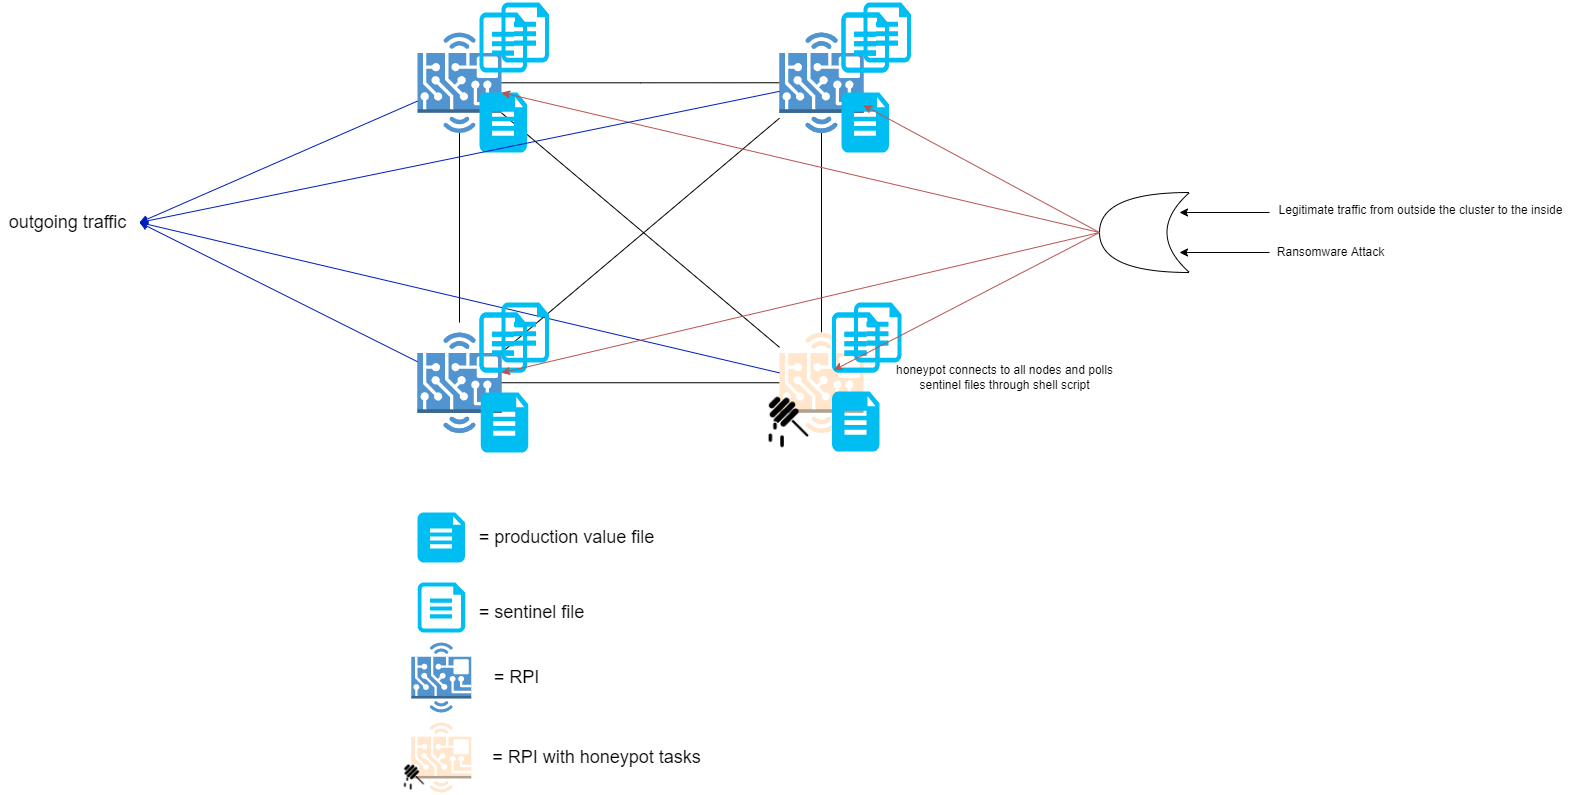
\includegraphics[width = 16cm]{images/ramsonwareHoneypot.png}
  \caption{ Example scenario of honypot against ramsonware attacks.}
  \label{fig:irradiances}
\end{figure}
\FloatBarrier

\subsubsection{Cluster}

\noindent Any Raspberry Pi in the picture represents a server, each connected to more clients (e.g., sensor nodes, not shown in the picture). Such servers are then connected among each other through a network and a communication protocol.\\
In this example, the architecture of the network is a full mesh, implying that each server is directly connected to any other. You could think of this network as either a local area network (LAN) or wide area network (WAN). They offer two different flavors of the same problem since in LANs you assume that all devices belonging to the network own a different local IP address and you should deal with the NAT system, while in a WAN servers have different public IP addresses and you should deal with DNS in order to communicate with each node in the network. \\ 
Raspberry devices exchange messages via MQTT, a lightweight publish/subscribe protocol. \\
Each device can manage messages of two kinds:

\begin{itemize}
 \item Dispatched commands. They should arrive from the dispatcher in the network (not shown here). The ransomware will pretend to be the dispatcher to let a victim device execute malicious encryption;
  \item Attack notifications. If under attack, a device broadcasts a message stating that is the victim of an attack in progress.
\end{itemize}


\subsubsection{Defensive Mechanism}

\noindent Each raspberry stores both files that are needed for the various operations it has to perform (e.g., files storing data from sensors) and files that are useless to the purpose of the cluster. The latter ones are better known as "sentinel files". Nobody should ever interact with sentinel files since they are useless for benign purposes, thus every modification to them must be considered as malicious.\\
Each raspberry runs a periodic check on the status of its own sentinel files, by checking their hash digest. If a mismatch takes place, then an attack notification is broadcasted and the node performs a shutdown, both avoiding to encrypt all its file system and avoiding to infect other nodes in the cluster. This operation is crucial, it grantes that the ransomware cannot spread out of the victim's file system. \\
The infected raspberry is inserted in a blacklist by all other nodes in the cluster, its messages are not read anymore because they are considered malicious. The node is deleted from the blacklist after a fixed amount of time. During this interval, a technician is supposed to perform a reset of the infected device.\\
Masking (or redirection) of some linux commands is provided to help sentinel files always appear as first encountered by the ransomware. Masking is provided for some options of commands "ls", "sort" and "rm" that could affect the order thanks to which files are displayed in a directory.

\subsubsection{Ransomware}

\noindent Most real ransomware would have been too harmful and many of them could have put our systems in danger. We chose to build our own ransomware that claims to be the dispatcher and sends messages (containing bash commands) to a victim in the cluster. \\
Ransomware aim at encrypting the victim's file system thanks to asymmetryc encryption. They try to encrypt the victim's file system with their own public key, obliging the victim to restore data by applying decryption with the ransomware's private key, that is secret until a payment is received.
Our ransomware performs the following steps:
\begin{enumerate}
  \item Creation of a pair of asymmetric keys;
  \item Injection of the public key in the victim's file system;
  \item Encryption, directory by directory, of each file in the victim's file system using the public key.
\end{enumerate}




\section{Case of study 2: Cluster and Honeypot for a DoS attack}

For this solution we took a cue from the paper \textit{Use of Honeypots for Mitigating DoS Attacks 
targeted on IoT Networks}\cite{7944057} where we found an analysis of the usage of a honeypot to reduce the damage of a DOS attack. One of the several possible attacks on IoT 
systems, Denial of Service (DoS) attack has been a nightmare for 
communication networks over the years and they 
pose a major security threat to IoT systems as well.\\
\subsection{Goal of the project}

The goal in this part of the project is to structure a tree cluster and elaborate an honeypot able to protect it from a DOS attack 
focusing on the IoT aspect of the project and make the solution really usable by these small devices.
  
\subsection{Solution overview: DOSPOTPY and climatOffice}
In the last years it becomes more and more important to avoid waste of energy at home and at work, due to the increasing cost of energy and to the environmental impact from the chain of the energy supply. So a startup develop a new IoT system named climatOffice(This is only an imaginary company, it doesn't exist in the real life). This solution aims at control the temperature in every office of the company, using N temperature sensors in every room an at least one air conditioner. The desired temperature could be set by an external terminal to the server that control every room. If there are windows in the room, the system also offer the possibility to control the illumination using automatics roll-up shutter. The last feature of this IoT cluster is to possibly control the accesses to some vulnerable rooms, like the server's farm room. So it can lock or unlock some doors. It can do this last thing automatically or by a command from a terminal. A possible Dos attack could for example avoid the door to close or open, or shut down the air conditioner system. To avoid so we could implement our systemr like in the figures below.
\begin{figure}[h!]
  \centering
  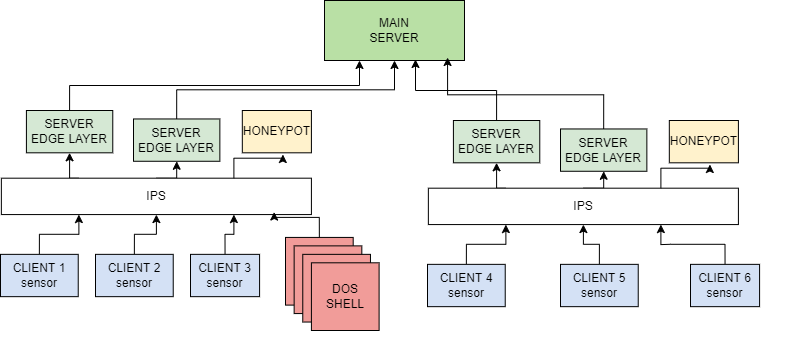
\includegraphics[width = 10cm]{images/IOTlever2IPS.png}
  \caption{An example of the climatOffice IoT cluster}
  \label{fig:TCPDos}
\end{figure}
\FloatBarrier
\noindent
The cluster consists of a main server to which the various edge servers are connected so a client  from the outside will turn out to be the leaf of this tree that can also evolve in multiple layers, in this case we preferred to remain fairly simple. The dispatcher, once the client sends a packet, redirects it to the server it is interacting with, every time a new connection arrives the dispatcher evaluates it as "harmful" then sends all the packets to the honeypot which, while the dispatcher continues the his job, checks that this client is credible and redirects the response to the dispatcher so that he is free to create a new connection with one of the servers. When a client is malicious (it sends too many packets, or with an unconfirmed structure) the honeypot writes the IP to a blacklist and then the dispatcher silences the connection, so the DOS attacker will seem to be sending data but actually can't slow down the system. In a litle system we could think of one dispatcher that manage all the servers indeed for a more larger one ,to better deliver the traffic and have less delay, is a good choice to have more than one dispatcher each one that manage a part of the cluster.\\
 For example, our attacker implement a bot that connect to the system and create thousands of fake temperature sensor that send random and wrong data to the server. Our dispatcher usually send new traffic connection to the honeypot, that will analyse the data . If this is no sense data, the honeypot will store in a log file(black list) the IP addresses of the fake sensor and will told to the dispatcher  to avoid accept new packets from that IP.
In a more simple way of cluste rwe can think of having much fewer packets and therefore of having less traffic in the dispatcher, if so we can then merge the dispatcher and the honeypot so that the check is faster without fill the dispatcher too much.

\subsection{The dispatcher evolution: IPS issue}

In order to build our cluster we have starting from the structures gives by the paper that is shown below:\\

\begin{figure}[h!]
  \centering
  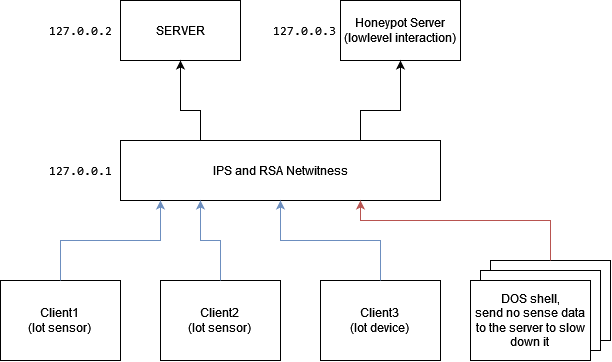
\includegraphics[width = 15cm]{images/IOTIPS.drawio.png}
  \caption{IoT network scheme with IPS.}
  \label{fig:2period}
\end{figure}
\FloatBarrier
In this first draft, which was then elaborated to arrive at the solution used in the implementation, we pay particular attention to the  Intrusion Prevention System (IPS) that is an active protection system. It attempts to identify potential threats based upon monitoring features of a protected host or network and can use signature, anomaly, or hybrid detection methods. Unlike an Intrusion Detection System, an IPS takes action to block or remediate an identified threat. While an IPS may raise an alert, it also helps to prevent the intrusion from occurring. An IDS is a passive monitoring solution for detecting cybersecurity threats to an organization. If a potential intrusion is detected, the IDS generates an alert that notifies security personnel to investigate the incident and take remedies against the action. \\
In our very first proposal the system is less complex, because the IPS itself takes the decision on where to redirect the traffic to. If it is a malicious packet, to the honeypot that will collect data about it, if it is a normal one, to the server. The IPS needs time to take decisions, so the traffic could be slowed down by it. If the application doesn't require high availability, this solution is acceptable.
Our second idea is reported in figure below.

\begin{figure}[h!]
  \centering
  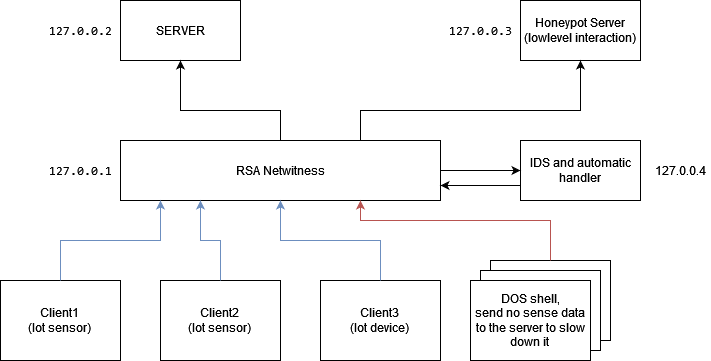
\includegraphics[width = 15cm]{images/IOTIDS.drawio.png}
  \caption{IoT network scheme with IDS.}
  \label{fig:1period}
\end{figure}
\FloatBarrier

This time an ad-hoc server has an IDS, that arises an alarm when something wrong is happening. Then an algorithm inside the server takes a decision on what to do with this possible malicious connection, and sends a command to the RSA server to redirect the traffic. In this way, the system has an high availability because the RSA server is not slow down by the IDS, that acts in a totally autonomous way. However, this idea requires more engineering effort and hardware so we redirect the solution to a more simple IPS to create a more realistic IoT cluster like in the figure below. 
\begin{figure}[h!]
  \centering
  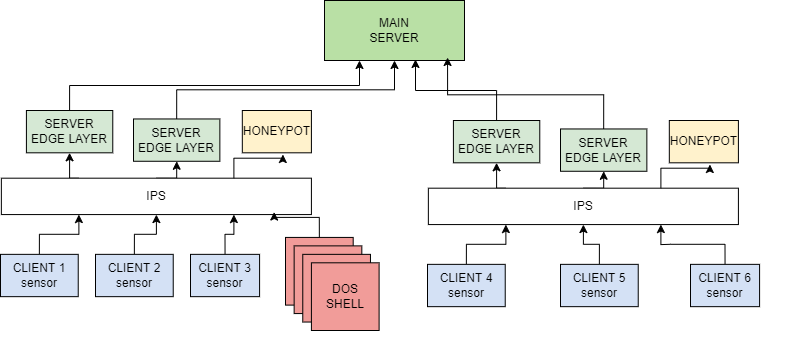
\includegraphics[width = 15cm]{images/IOTlevel2IPS.drawio.png}
  \caption{IOT network scheme level 2 with dispatcher}
  \label{fig:3period}
\end{figure}
\FloatBarrier
 In this solution all the traffic generated by the clients is redirected to the various servers that the IPS serves, when an attack occurs It knows it by checking if it is a new IP or if the structure of the packets is wrong and redirect the traffic to the honeypot. 
In a second look we noticed that IPS was simple and much more like a dispatcher redirecting packets, thats why in our implementations there is a dispacher. In our implementation there is only one dispacher and one honeypot because the cluster is simple, but the number of honeypots and cluster could vary, depending of the number of sensors and servers.










